%\documentclass[11pt]{article}\usepackage{amssymb,amsmath,amsthm,hyperref,verbatim,pict2e,graphicx,array,listings,appendix,color}
\usepackage{algorithm,algorithmic,booktabs,marvosym,wrapfig,xytree,multicol,multirow,arydshln,nameref}
\hypersetup{colorlinks,citecolor=black,filecolor=black,linkcolor=black,urlcolor=black
	%pdfborderstyle={/S/U/W 1},urlbordercolor=1 0 0,linkbordercolor=.5 1 1, citebordercolor=.5 1 1
}
\usepackage[usenames]{xcolor} % color names ,dvipsnames,svgnames,table
\usepackage[utf8]{inputenc}
\usepackage[T1]{fontenc}
\usepackage[english]{babel}

% margins
\pagestyle{headings}
\oddsidemargin 0.0cm
\evensidemargin 0.0cm
\topmargin 0.0cm
\headheight 0.0cm
\headsep 1.0cm
\textheight 22.0cm
\textwidth 16.0cm
\parskip 0.1cm
\parindent 0.0cm
\footskip 1.0cm

% compact titles
\usepackage[compact]{titlesec}
\titlespacing{\section}{0pt}{8pt}{0pt}
\titlespacing{\subsection}{0pt}{8pt}{0pt}
\titlespacing{\subsubsection}{0pt}{8pt}{0pt}

% compact lists
\usepackage{enumitem}
\setitemize{noitemsep,topsep=0pt,parsep=0pt,partopsep=0pt}
\setenumerate{noitemsep,topsep=0pt,parsep=0pt,partopsep=0pt}
\def\ul{\begin{itemize}}
\def\ule{\end{itemize}}
\def\ol{\begin{enumerate}}
\def\ole{\end{enumerate}}

% misc
\def\up#1{\textsuperscript{#1}}
\def\quote#1{\par\begingroup\leftskip1em\rightskip\leftskip\textit{#1}\par\endgroup}


% listings
\definecolor{dkpink}{RGB}{200,0,100}
\definecolor{gray}{RGB}{128,128,128}
\lstset{
	xleftmargin=20pt,
	numberstyle=\tiny,stepnumber=1,numbersep=5pt,
	showstringspaces=true,         % underline spaces within strings
	tabsize=2,                      % sets default tabsize to 2 spaces
	captionpos=t,                   % sets the caption-position to bottom
	breaklines=true,                % sets automatic line breaking
	breakatwhitespace=true, % sets if automatic breaks should only happen at whitespace
	title=\lstname, % show the filename of files included with \lstinputlisting; also try caption instead of title
	basicstyle=\small\tt,keywordstyle=\color{blue},commentstyle=\color{gray},stringstyle=\color{dkpink}
}
% define Scala syntax
\lstdefinelanguage{Scala}{
	morekeywords={abstract,case,catch,class,def,do,else,extends,false,final,finally,for,if,implicit,import,%
	match,mixin,new,null,object,override,package,	private,protected,requires,return,sealed,super,this,%
	throw,trait,true,try,type,val,var,while,with,yield},
	otherkeywords={=>,<-,<\%,<:,>:,\#,@},sensitive=true,
	morecomment=[l]{//},	morecomment=[n]{/*}{*/},
	morestring=[b]",morestring=[b]',morestring=[b]"""
}

% title page
\makeatletter
\gdef\@subtitle{}\def\subtitle#1{\gdef\@subtitle{#1}}
\def\my@heading{
\def\ps@headings{\let\@mkboth\markboth
	\def\@evenhead{\small \rightmark \hfill \textit{\@title}, p.~\thepage}
	\def\@oddhead{\@evenhead}}\pagestyle{headings}}
\renewcommand{\maketitle}{
	%\begin{titlepage}
	\setcounter{page}{0}\thispagestyle{empty}
	{\centering\null\vfill
\includegraphics[width=5.5cm]{inc/logo_epfl.pdf} % EPFL logo
	\vspace{1.5cm}\hrule \vspace{2.5cm} {\LARGE \@title \par} {\large \emph \@subtitle \par}
	\vspace{2.75cm} {\Large \@author \par}
	\vspace{5.5cm} {\large School of Computer and Communication Sciences, EPFL \par}
	\vspace{1.0cm} {\@date \par} % date
	\vfill\null\par}\my@heading
	\newpage
	%\end{titlepage}
}
\newcommand{\shorttitle}{
	\thispagestyle{empty}
	\hfill 
\includegraphics[width=3cm]{inc/logo_epfl}\vspace{.1cm} % EPFL logo
	\begin{center} {\LARGE \@title} \\ \vspace{.1cm} {\large \textit{\@subtitle}} \\ \rule[1ex]{350pt}{.5pt} \\
	\@author \\ {\small School of Computer and Communication Sciences, EPFL} \vspace{.2cm} \\{\small \@date}
	\end{center} \vspace{.5cm}\my@heading
}
\makeatother

% new XeTeX title page
\usepackage[T1]{fontenc}
\usepackage{fontspec}
\newfontfamily\fonth{Helvetica}
\newfontfamily\fonthn{Helvetica Neue}
\newfontfamily\fonthc{Helvetica Neue Condensed Bold}
\newfontfamily\fonthl{Helvetica Neue UltraLight}

\makeatletter
\renewcommand{\maketitle}{
	%\begin{titlepage}
	\setcounter{page}{0}\thispagestyle{empty}
	\hfill 
\includegraphics[width=8.5cm]{inc/logo_epfl.pdf} \vfill
	{\fontsize{25pt}{11pt}\fonthc Master project report \vspace{0.5cm}} \\
	{\fontsize{40pt}{11pt}\fonthl \@title} \vspace{0.2cm} \\ {\fontsize{20pt}{11pt}\fonthl \@subtitle} \\
	\vspace{1.5cm} \\
	{\begin{tabular}{ll}
	Laboratory	& Programming Methods Laboratory, LAMP, EPFL \\
	Professor		& \href{mailto:martin.odersky@epfl.ch}{Martin Odersky} \\
	Supervisors	& \href{mailto:vojin.jovanovic@epfl.ch}{Vojin Jovanovic}, \href{mailto:manohar.jonnalagedda@epfl.ch}{Manohar Jonnalagedda}   \\
	Expert		& \href{mailto:mirco.dotta@typesafe.com}{Mirco Dotta}, Typesafe \\
	Student		& \href{mailto:thierry.coppey@epfl.ch}{Thierry Coppey} \\
	Semester		& Autumn 2012 \\
	\end{tabular}}
	\my@heading
	\newpage
	%\end{titlepage}
}
\makeatother

% appendix
\makeatletter
\let\origappendix\appendix
\renewcommand\appendix{\clearpage\pagenumbering{Roman}\origappendix\section*{\appendixname}\lstset{frame=tb,numbers=left}}
\makeatother

% default
\author{\href{mailto:thierry.coppey@epfl.ch}{Thierry Coppey}} %, \href{mailto:manohar.jonnalagedda@epfl.ch}{Manohar Jonnalagedda}, \href{mailto:nithin.george@epfl.ch}{Nithin George}
\begin{document}

\section{Benchmarks} \label{benchmarks}
In an attempt to provide realistic benchmarks, we tried to gather state-of-art implementations. The authors of \cite{gpu_atlp} did not respond to our multiple solicitations. The authors of \cite{swat_mega} were very friendly and provided us their source code. Unfortunately, since they address a different category of problem (Smith-Waterman on huge sequences whereas we focus on smaller non-serial problems) their implementation might be biased towards large sequences, and leverage problem-specific information (wavefront) that our implementation cannot address. Finally, we asked lately the authors of \cite{gpu_rnafold} who did not respond either to our solicitations. The authors of \cite{gapc_thesis} kindly share their implementation on a dedicated website\footnote{\url{http://www.gapc.eu}}.

We organize the benchmarks as follow: if we have at our disposal a working implementation that could be run on our evaluation platform, we use it, otherwise, we refer to the related paper and rescale the part of the result corresponding to memory accesses according to the memory bandwidth of the related device so that we can have a good approximation of how they could compare.

\subsection{Metrics} \label{metrics}
The main metrics of interest is the running time. In an attempt to reduce the variance, we would like to run multiple consecutive test and take the median running time, since the median is less sensitive to outlier than the average\cite{perfeval}. Unfortunately, several factors hampers these ideal conditions. First the variance in the running time of CUDA kernels might be significant, in particular for short running time. This is due to the fact that the GPU needs to be 'warmed-up' before actual computation can happen. Similarly, the JVM is also subject to running time variance that is mainly due to the garbage collection\footnote{\url{http://www.oracle.com/technetwork/java/javase/gc-tuning-6-140523.html\#cms.overhead}} and JIT optimizations \cite{java_jit}.

Also the input and problem might introduce variance. As example, we can consider two extreme cases: matrix chain multiplication and Zuker RNA folding, with a test environment of 100 random inputs (of length respectively 512 and 80) and a GPU warmup of 10 computations. In this settings, matrix chain multiplication computations are executed in a perfectly constant time\footnote{With respect to truncation and measurment accurcy, has less than 1\% of variation (not observable).} (0.127 seconds), which mean that we sufficiently reduced the noise. Oppositely, the Zuker RNA folding running times appear much more scattered as presented below:

\begin{figure}[H]\begin{center}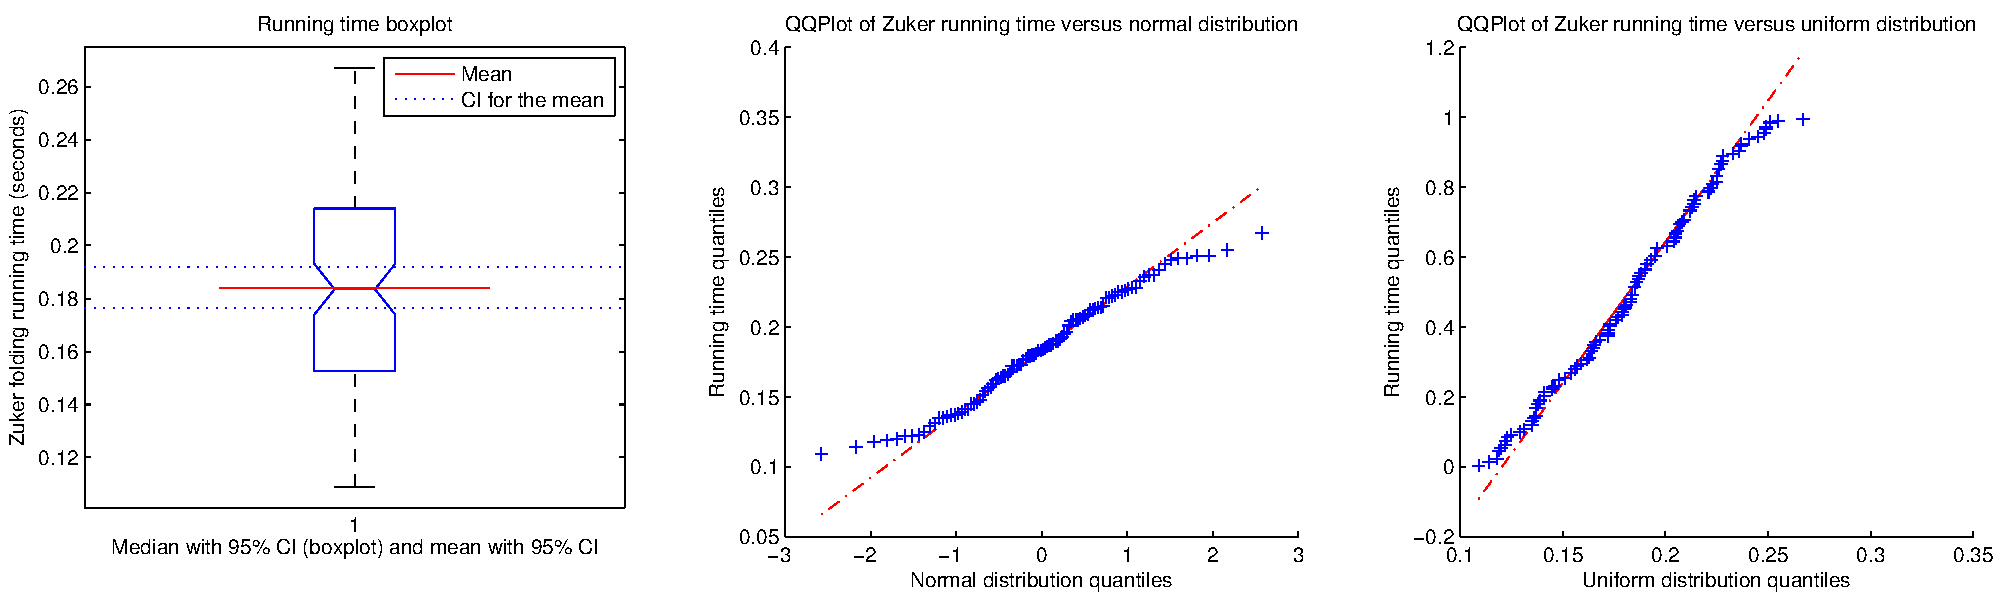
\includegraphics[width=16cm]{inc/var_zuker.pdf}\end{center}
\caption{Zuker folding running time (seconds). Quartiles: 0.152, 0.183 (median), 0.214}\label{fig:var_zuker}\end{figure}

Using the QQplot\footnote{Quantile-to-quantile plot, used to compare two distributions against each other.}, the distribution is heavily tailed (has more results towards the ends of the range) than a Gaussian distribution (fig.~\ref{fig:var_zuker} center) but fits better an uniform distribution (fig.~\ref{fig:var_zuker} right). If we run multiple time the program over the same input, we obtain the same behavior as with the matrix multiplication (strictly identical time); hence we can conclude that Zuker is an input sensitive problem whereas matrix chain multiplication is not. It follows that we need to be careful to test with exactly identical input set different implementations.

As the device memory is quite limited, it seems interesting to also take into account the space usage. The space requirement limits the maximal size of addressable problems  on a particular hardware. This might be a concern for large problems, because they would require special adaptation to handle such cases both correctly and efficiently. However, this metric heavily depends on the problem and simple solutions like using a device with larger memory or using main memory (if a $5\times$ slowdown is still acceptable) could solve this issue, hence we do not consider this metric hereafter (except as an upper bound on the dimension of the input).

\subsection{Benchmarking platform}
Our benchmarking platform is an Apple notebook with a Core i7-3720QM with 16Gb of main memory and an NVIDIA GeForce GT 650M running under MacOS X 10.8 and Oracle JDK 1.7.0-10. A workaround (see listing~\ref{cpu_workaround}) allows us to use the CPU to render the user interface while leaving the graphic card available to execute CUDA kernels. Unfortunately, due to impossibility to disable the watchdog timer in MacOS, CUDA kernels are limited to few seconds of running time before they are automatically aborted.

% ----------------------------------------------
% MatrixMult-512, Mac+JDK7
% -> Original: 24.658 sec
% -> Optimized concatenation: 18.924 sec
% -> Tabulation as arrays+inline: 14.849 sec
% -> Re-optimized concatenation: 10.76 sec
% ----------------------------------------------
\def\hh{\normalsize\bf}
\def\hl#1#2{\begin{minipage}{3.5cm} {\bf #1} \\[-2pt] \footnotesize #2 \vspace{6pt} \end{minipage}}
\def\hdps{\hl{DynaProg}{Scala parsers}}
\def\hdpc{\hl{DynaProg}{CUDA parsers}}
\def\hdpcz{\hl{DynaProg}{CUDA-Zuker}}
\def\hdpcr{\hl{DynaProg}{CUDA-RNAfold}}
\def\hhoc{\hl{Optimized}{C, single thread}}
\def\hhog{\hl{Optimized}{CUDA, 64-bit}}
\def\hgapc{\hl{GAPC}{\cite{gapc_thesis}, C, single thread}}
\def\hatlp{\hl{ATLP}{\cite{gpu_atlp}, rescaled results$^{(1)}$}}
\def\hcua{\hl{CUDAlign}{\cite{swat_linear}, version 2.0}}
\def\hvien{\hl{ViennaRNA}{\cite{vienna_rna}}}
\def\hrna{\hl{RNAfold}{\cite{gpu_rnafold}}}

\def\hcpu{\midrule \multirow{4}{*}{\rotatebox{90}{\normalsize\bf CPU $\quad$}}}
\def\hgpu{\midrule \multirow{4}{*}{\rotatebox{90}{\normalsize\bf GPU $\quad$}}}

\subsection{Matrix chain multiplication}
% CPU: DynaProg(Scala), hand optimized C, GAPC and ADPFusion
% GPU: GPU: DynaProg(CUDA), hand optimized CUDA, ATLP and GAPC-OpenCL?
We have seen previously that this problem is not input sensitive in (\S\ref{metrics}), hence we can safely use different random number generators among different implementations without compromising the validity of the results.  Also note that the hand-optimized results are slightly worse than those presented in (\S\ref{baseline_impl}), this is caused by enabling the 64-bit mode. Since external libraries linked with the Java virtual machine must be in 64 bit, we also enabled this mode in hand-optimized version to maintain a fair comparison, thereby slightly reducing the performance of CUDA operations.

\begin{table}[H]\begin{center}{\small\begin{tabular}{llrrrrrrr}\toprule
&\hh  Matrix dimension &\hh 64 &\hh 128 &\hh 192 &\hh 256 &\hh 384 &\hh 512 &\hh 768 \\ \hcpu
& \hdps	& 0.05	& 0.20	& 0.80	& 2.03	& 6.65	& 15.10	& 47.40	\\
& \hhoc	& <0.01	& <0.01	& <0.01	& 0.01	& 0.03	& 0.08	& 0.28	\\
& \hgapc	& 0.01	& 0.01	& 0.03	& 0.05	& 0.15	& 0.35	& 1.16	\\[-2pt] \hgpu
& \hdpc	& 0.03	& 0.04	& 0.05	& 0.07	& 0.13	& 0.13	& 0.21	\\
& \hhog	& <0.01	& 0.01	& 0.01	& 0.02	& 0.04	& 0.08	& 0.17	\\
& \hatlp	& 0.17	&	 	&		& 0.20	& 		& 0.23	& 		\\
\midrule
&\hh Matrix dimension &\hh 1024 &\hh 1536 &\hh 2048 &\hh 3072 &\hh 4096 &\hh 6144 &\hh 8192 \\ \hcpu
& \hdps	& 109.77	& 368.21	& 877.30	& 3059.42 & 		& 		& 		\\
& \hhoc	& 1.18	& 7.06	& 19.81	& 78.90	& 206.56	& 799.53	& 2010.49 \\
& \hgapc	& 2.82	& 10.02	& 25.16	& 91.69	& 224.70	& 		&  		\\[-2pt] \hgpu
& \hdpc	& 0.35	& 0.85	& 1.69	& 4.79	& 10.32	& 31.60	& 71.22	\\
& \hhog	& 0.32	& 0.82	& 1.65	& 4.74	& 10.35	& 31.94	& 72.38	\\
& \hatlp	& 0.40	& 0.74	& 1.33	& 3.43	& 7.29	& 		& 		\\
\bottomrule\end{tabular}}\end{center}\caption{Running time of matrix chain multiplication (in seconds)}\end{table}

$^{(1)}$ Assuming that 72\% of the running time is due to memory accesses, and considering a $3.55\times$ memory throughput slowdown of the original results (see \S\ref{results_discussion}). % 0.06 & 0.07 & 0.08 & 0.14 & 0.47 & 2.57 => f[x_] := (x*(1 - .72)) + (x*0.72)*(102.4/28.8)
% 0.1704 & 0.1988 & 0.2272 & .3976 & 1.3348 & 7.2988

The running time of DynaProg/CUDA includes the overhead of back and forth JNI conversion (scales linearly between 0.018 and 0.057 seconds) but does not include the overhead due to the code generation which decomposes in 0.068 seconds for analysis and code synthesis (once per algebra/grammar pair) and 0.086 + 1.753 seconds for respectively Scala and CUDA compilation (constant time, once per problem dimension). These execution time results are presented similarly for the following problems.

For DynaProg/Scala we use a variant of the problem description: the original version only stores the matrix multiplication score whereas the modified version also stores the matrix dimension. This allows a speedup of $2.9\times$ probably due to the additional lookups overhead. Also with the default JVM parameters, the program cannot address sequences longer than $\sim 420$ elements due to a stack overflow, for these benchmarks, we increased this limit.

From the results we see that this problem is well suited for GPUs where the computation pattern is very regular across threads. In this case, the generated CUDA code produces performance that is comparable to hand-optimized CUDA code, and comparable to one of the state of the art implementation with less than $1.5\times$ performance degradation. ATLP leverages the regularity of the access pattern optimize the resource utilization and adaptively map subproblems\cite{gpu_atlp}. As we cannot benefit of such problem-specific knowledge, our approach is to compute elements independently and synchronize efficiently.

\subsection{Smith-Waterman (affine gap cost)}
% CPU: DynaProg(Scala), hand optimized C, GAPC and ADPFusion
% GPU: DynaProg(CUDA), hand optimized CUDA, CUDAlign
Smith-Waterman with affine gap cost is a serial problem, which is not directly the focus of our project but nevertheless can be addressed efficiently. The problem formal description (\S\ref{swat_affine}) uses 3 matrices. However, since two of these matrices only propagate information along line or column, it is possible to encode this information in a wavefront (see \S\ref{calc_simplifications}) instead of maintaining it in a memory-expensive matrix. This knowledge is leveraged by \cite{ATLP}, however, in our case, we cannot describe the wavefront in the grammar and need to maintain explicitly 3 matrices, thereby multiplying by 3 the memory usage\footnote{Actually slightly less than 3 because we replace 2 matrices in $O(n^2)$ by two vectors in $O(n)$}.

\begin{table}[H]\begin{center}{\small\begin{tabular}{llrrrrrrr}\toprule
&\hh  Matrix dimension &\hh 64 &\hh 128 &\hh 192 &\hh 256 &\hh 384 &\hh 512 &\hh 768 \\ \hcpu
& \hdps	& 0.04	& 0.13	& 0.27	& 0.48	& 1.07	& 1.92	& 4.33	\\
& \hhoc	& <0.01	& <0.01	& <0.01	& <0.01	& <0.01	& <0.01	& 0.01	\\
& \hgapc	& 0.01	& 0.01	& 0.01	& 0.01	& 0.02	& 0.03	& 0.06	\\[-2pt] \hgpu
& \hdpc	& 0.03	& 0.03	& 0.03	& 0.04	& 0.05	& 0.05	& 0.06	\\
& \hhog	& 0.00	& 0.00	& 0.00	& 0.00	& 0.00	& 0.00	& 0.00	\\
& \hcua	& 0.11	& 0.12	& 0.07	& 0.07	& 0.07	& 0.07	& 0.13	\\
\midrule
&\hh Matrix dimension &\hh 1024 &\hh 1536 &\hh 2048 &\hh 3072 &\hh 4096 &\hh 6144 &\hh 8192 \\ \hcpu
& \hdps	& 7.84	& 18.95	& 33.63	& 70.86	& 		& 		& $^{(2)}\infty$ \\
& \hhoc	& 0.01	& 0.02	& 0.04	& 0.10	& 0.17	& 0.40	& 0.71	\\
& \hgapc	& 0.10	& 0.22	& 0.39	& 0.91	& 1.62	& 4.41	& 11.20 	\\[-2pt] \hgpu
& \hdpc	& 0.07	& 0.11	& 0.15	& 0.13	& 0.20	& 0.32	& $^{(1)}$3.21 	\\
& \hhog	& 0.01	& 0.02	& 0.02	& 0.04	& 0.07	& 0.14	& 0.27	\\
& \hcua	& 0.13	& 0.15	& 0.14	& 0.14	& 0.15	& 0.17	& 0.20 	\\
\bottomrule\end{tabular}}\end{center}\caption{Running time of Smith-Waterman (in seconds)}\end{table}

$^{(1)}$ Since the memory requirements are larger than the device capacity, the backtrack matrix overflows in the main memory, thereby significantly degrading the performance. This extra memory requirement is due to the use of 3 matrices to avoid the non-serial dependencies (hence requiring at least $3 \cdot 2$ bytes of memory per matrix element for backtrack).

$^{(2)}$ Extremely little progress due to intensive JVM garbage collection after some delay, even by tuning the JVM parameters ({\tt -Xss512m -Xmx12G -Xms12G}), and independently of whether top-down or bottom-up parsing approaches are taken. After a minute, most of the time is spent in (full) garbage collections. In this algorithm, the aggregation function application contributes to approximately 30\% of the total running time.

From these result, it is possible to say that although not being the primary focus, the serial problem can be solved efficiently as well in our framework, assuming that the device memory is sufficiently large to store all the matrices. We might attribute the proportional overhead of our implementation (compared to the optimized version) to the additional verifications for result cell emptiness (these are hidden in matrix multiplication by the memory accesses). Removing them requires problem-specific knowledge (for example setting an infinite value), as described in \S\ref{normalization}.

\subsection{Zuker RNA folding}
% CPU: DynaProg(Scala), GAPC, ADPFusion and ViennaRNA
% GPU: DynaProg(CUDA), RNAFold?/Lavenier VS ViennaRNA-OpenCL?, GAPC-OpenCL?
The Zuker RNA folding algorithm significantly differs from the two previous problems because it relies on energy functions involving experimental parameters (constants). These parameters are encoded in lookup tables that need to be accessed usually at multiple places in each energy function. Additionally, energy functions involve conditions and possibly loops hence are more complex than the simple regular patterns of matrix multiplication and Smith-Waterman, thereby introducing possible thread divergence that reduces the performance.

For this problem, we present two grammar variants. The Scala version and CUDA-Zuker share the same grammar as GAPC\cite{gapc_thesis}, which is more complex than the RNAfold grammar, that is shared by the two implementation with the same name. Although not stated explicitly in the paper \cite{gpu_rnafold}, this implementation limits the size of internal loops to 30 (following current practice in the domain \cite{rna_structure}). Limiting the size of the internal loops allows to reduce the running time complexity from $O(n^4)$ to $O(n^3)$, because large loops rarely occur in practice \cite{rna_structure}.

\begin{table}[H]\begin{center}{\small\begin{tabular}{llrrrrrrr}\toprule
&\hh  Matrix dimension &\hh 64 &\hh 128 &\hh 192 &\hh 256 &\hh 384 &\hh 512 &\hh 768 \\ \hcpu
& \hdps	& 0.07	& 0.67	& 2.26	& 4.98	& 17.61	& 39.44	& 130.71	\\
& \hvien	& 0.01	& 0.01	& 0.02	& 0.03	& 0.07	& 0.12	& 0.29	\\
& \hgapc	& 0.01	& 0.03	& 0.07	& 0.13	& 0.41	& 0.93	& 2.89	\\[-2pt] \hgpu
& \hdpcz	& 0.13	& 0.48	& 0.88	& 1.41	& 2.84	& 4.55	& 8.51	\\
& \hdpcr	& 0.17	& 0.54	& 0.92	& 1.33	& 2.25	& 3.22	& 5.34	\\
& \hrna	& 0.06	& 0.11	& 0.14	& 0.20	& 0.44	& 0.80	& 1.89	\\
\midrule
&\hh Matrix dimension &\hh 1024 &\hh 1536 &\hh 2048 &\hh 3072 &\hh 4096 &\hh 6144 &\hh 8192 \\ \hcpu
& \hdps	& 306.12	& 1036.78 &		& 		& 		& 		& 	 	\\
& \hvien	& 0.57	& 1.53	& 3.19	& 9.37	& 20.18	& 59.65	& 133.65 	\\
& \hgapc	& 6.66	& 22.91	& 56.97	& 208.33	& 529.40	& 		&  		\\[-2pt] \hgpu
& \hdpcz	& 13.61	& 30.45	& 56.22	& 152.88	& 365.24	& 		& 		\\
& \hdpcr	& 7.68	& 15.89	& 26.43	& 66.30	& 153.90	& 		& 		\\
& \hrna	& 3.52	& 9.08	& 19.59	& 67.32	& 163.14	& 		& 		\\
\bottomrule\end{tabular}}\end{center}\caption{Running time of Zuker RNA folding (in seconds)}\end{table}

These results are interesting because they demonstrate that for complex problems, the GPU do not behave as good as we wished compared to the CPU (comparing ViennaRNA and RNAfold). Beside that, we can notice that for large sequences, our Zuker grammar GPU implementation is on par with GAPC, and the RNAfold grammar is on par with the RNAfold implementation, although we might argue that the purpose of RNAfold is slightly different (using synergistically CPU and GPU to fold multiple small sequences of RNA).

%\end{document}
